%% BAN TIENG VIET de DOC/DUYET. Ban nop la main.tex (tieng Anh).
%% Moi con so, nhan (label), tham chieu, bang va hinh GIU Y NGUYEN nhu main.tex -> doi chieu duoc.
%%
%% >>> Bien dich pdfLaTeX. Neu dau tieng Viet loi, doi sang XeLaTeX va thay 3 dong font bang:
%%     \usepackage{fontspec}\usepackage{polyglossia}\setmainlanguage{vietnamese}
\documentclass[preprint,12pt]{elsarticle}

\usepackage{lmodern}
\usepackage[utf8]{inputenc}
\usepackage[T5]{fontenc}
\usepackage[vietnamese]{babel}

\usepackage{amsmath,amssymb}
\usepackage{booktabs}
\graphicspath{{figures/}{./}}

\journal{Results in Engineering}

\begin{document}
\begin{frontmatter}

\title{Đếm nhân tế bào với một phần tám chi phí chú thích:
nhãn mức ảnh sánh ngang mặt nạ mức điểm ảnh}

\author[uit]{Viet Hang Duong}
\ead{hangdv@uit.edu.vn}

\author[uit]{Thi Thu Hiep Dinh\corref{cor1}}
\ead{dinhthithuhiep1@gmail.com}
\cortext[cor1]{Tác giả liên hệ.}

\affiliation[uit]{organization={Khoa Khoa học Máy tính, Trường Đại học Công nghệ Thông tin (UIT), ĐHQG-HCM},
            city={Thành phố Hồ Chí Minh},
            country={Việt Nam}}

\begin{abstract}
Việc triển khai một hệ định lượng nhân tế bào tự động trên thực tế bị giới hạn bởi hai ràng buộc kỹ thuật hơn là
bởi năng lực mô hình: công sức chuyên gia cần bỏ ra để chú thích dữ liệu huấn luyện, và yêu cầu rằng mọi con số
báo ra phải kèm một dung sai đã công bố. Chú thích mức điểm ảnh tốn hàng giờ công chuyên gia cho mỗi ảnh và mở
rộng kém sang mô, cơ quan hay trung tâm mới, thế nhưng phần lớn phương pháp đếm vẫn dựa trên phân đoạn, ước lượng
mật độ hoặc phát hiện, ngầm định rằng giám sát không gian dày đặc là điều kiện tiên quyết để đạt độ chính xác cao.
Bài báo kiểm định giả định đó một cách trực tiếp bằng một thí nghiệm có đối chứng, trong đó kiến trúc mạng, dữ
liệu và giao thức đánh giá được giữ cố định, còn kiểu giám sát là biến duy nhất. Chỉ với một con số đếm mức ảnh
làm nhãn, một mô hình 3,62 triệu tham số đạt $R^2$ bằng 0,918 trên PanNuke và vượt các đại diện được khảo sát của
phân đoạn, ước lượng mật độ và phát hiện trên cùng tác vụ đếm và cùng tập kiểm tra, dù cả ba đều đòi hỏi nhãn
định vị. Khi so giám sát bằng số đếm với giám sát bằng mặt nạ trên PanNuke, NuInsSeg và MoNuSeg, dấu của hiệu số
đảo chiều giữa các bộ dữ liệu, nên không chế độ nào ưu thế nhất quán. Trên PanNuke, lợi thế của giám sát bằng mặt
nạ có ý nghĩa thống kê nhưng bị chặn trên bởi một kiểm định tương đương ở mức 1,1\% số nhân trung bình mỗi ảnh,
trong khi nhãn đếm rẻ hơn ít nhất tám lần so với khoanh viền đầy đủ. Các thí nghiệm can thiệp có đối chứng giả cho
thấy mô hình phản ứng đặc hiệu với nội dung nhân, nhưng hình thành dự đoán bằng cách tích hợp bằng chứng trên toàn
ảnh chứ không phải bằng cách định vị từng thực thể. Bộ đếm thu được chạy trong $6{,}0$\,ms trên GPU và $46$\,ms
trên CPU, và các khoảng dự báo conformal có điều kiện theo cơ quan đạt độ phủ mục tiêu trên cả 19 loại mô. Do đó,
chú thích không gian dày đặc không phải là điều kiện tiên quyết để đếm nhân chính xác.
\end{abstract}

\begin{highlights}
\item Nhãn chỉ-đếm sánh ngang mặt nạ điểm ảnh cho bài toán đếm nhân trên ba bộ dữ liệu công khai
\item Kiểm định tương đương chặn khoảng cách ở 1,1\% số nhân trung bình mỗi ảnh, n = 2722
\item Nhãn đếm mức ảnh tốn chưa tới một phần tám chi phí khoanh viền đầy đủ mức điểm ảnh
\item Bộ đếm 3,62 triệu tham số chạy 6 ms trên GPU và 46 ms trên CPU ở kích thước 256x256
\item Khoảng conformal có điều kiện theo cơ quan giữ độ phủ mục tiêu trên cả 19 loại mô
\end{highlights}

\begin{keyword}
đếm nhân tế bào \sep chi phí chú thích \sep giám sát yếu \sep định lượng bất định \sep
dự báo conformal \sep thiết kế hệ đo \sep bệnh học tính toán
\end{keyword}

\end{frontmatter}

%%============================================================%%
\section{Giới thiệu}\label{sec:intro}

Số lượng và mật độ nhân tế bào là những chỉ số định lượng nền tảng trong bệnh học, phục vụ đánh giá tăng sinh,
phân độ khối u và phân tích vi môi trường mô. Phần lớn phương pháp học sâu hiện nay tiếp cận bài toán đếm nhân
một cách gián tiếp, bằng cách \emph{phân đoạn} hoặc \emph{phát hiện} từng nhân rồi suy ra số đếm từ kết quả đó.
Tuy chính xác, các phương pháp này đòi hỏi chú thích mức điểm ảnh hoặc mức thực thể, vốn tốn hàng giờ công chuyên
gia cho mỗi ảnh và mở rộng kém sang mô, cơ quan hay trung tâm mới.

Nhìn như một bài toán kỹ thuật, việc dựng một hệ như vậy tại một phòng xét nghiệm mới bị chi phối bởi ba ngân sách
hơn là bởi năng lực mô hình. Thứ nhất là \emph{ngân sách chú thích}: phần công sức chuyên gia phải mua trước khi
huấn luyện được mô hình đầu tiên, là khoản chi phí một lần lớn nhất và là khoản phải trả lại mỗi khi hệ được
chuyển sang cơ quan, phương pháp nhuộm hay trung tâm mới. Thứ hai là \emph{ngân sách tính toán} lúc suy luận, thứ
quyết định hệ có chạy được ngay cạnh máy quét hay chỉ chạy được trên phần cứng chuyên dụng. Thứ ba là một
\emph{đặc tả độ tin cậy}: một thiết bị báo ra con số mà không kèm dung sai thì không thể đặt vào trong một quy
trình ra quyết định, và một dung sai đúng trên trung bình nhưng hỏng ở vài loại mô cụ thể thì cũng không phải một
đặc tả dùng được. Bài báo xem việc chọn kiểu giám sát là một quyết định thiết kế dưới ba ngân sách đó, và đo xem
phương án rẻ nhất thực sự phải trả giá bao nhiêu.

Nằm dưới thông lệ hiện nay là một giả định hiếm khi được kiểm định trực tiếp: rằng muốn đếm chính xác thì phải
cung cấp cho mô hình \emph{vị trí} của từng nhân trong lúc huấn luyện. Trong khi giám sát chỉ bằng tổng số đối
tượng mức ảnh (\emph{chỉ-đếm}) đã được nghiên cứu nhiều ở bài toán đếm đám đông và một số bài toán đếm đối tượng
khác, việc đếm nhân trong bệnh học vẫn chủ yếu dựa vào chú thích không gian như điểm hoặc mặt nạ. Vì vậy, mức
giám sát tối thiểu mà bài toán đếm nhân thực sự đòi hỏi vẫn là câu hỏi mở, và kèm theo đó là quy mô ngân sách chú
thích mà một đợt triển khai phải dự trù.

Bài báo trả lời câu hỏi đó bằng một \emph{thí nghiệm có đối chứng}. Kiến trúc mô hình, dữ liệu và giao thức đánh
giá được giữ cố định, và biến thí nghiệm duy nhất là kiểu giám sát: mặt nạ mức điểm ảnh, hay một nhãn đếm cho mỗi
ảnh. Do đó mọi khác biệt quan sát được đều quy về \emph{chú thích}, không phải về dung lượng mô hình.
Hình~\ref{fig:design} trình bày thiết kế này và nêu kết cục của nó.

Các đóng góp chính như sau.
\begin{itemize}
\item Một nghiên cứu có đối chứng về ảnh hưởng của mức giám sát tới độ chính xác đếm, trên ba bộ dữ liệu độc lập
và một kiến trúc duy nhất. Không chế độ nào ưu thế nhất quán \emph{giữa các bộ dữ liệu}: dấu của hiệu số đảo
chiều, và trên tập kiểm tra lớn nhất, khoảng cách mà giám sát bằng mặt nạ nắm giữ, tuy có ý nghĩa thống kê, vẫn
bị chặn trên bởi kiểm định tương đương ở mức $1{,}1\%$ số nhân trung bình mỗi ảnh (Mục~\ref{sec:parity}).
\item Một phân tích cơ chế dựa trên thí nghiệm can thiệp có đối chứng giả khớp diện tích: dự đoán phụ thuộc đặc
hiệu vào nội dung nhân, nhưng đáp ứng lại dưới tuyến tính và bản đồ mật độ gần như không định vị nhân. Hai quan
sát này cùng nhau thu hẹp tập các cơ chế có thể giải thích kết quả nêu trên (Mục~\ref{sec:fidelity}).
\item Một so sánh với các đại diện của ba mô thức dùng nhãn định vị (phân đoạn, ước lượng mật độ và phát hiện)
trên cùng dữ liệu và cùng giao thức đánh giá: bộ đếm chỉ-đếm nhẹ đạt độ chính xác đếm cao hơn cả ba trong cấu
hình thông dụng của chúng, còn mô thức phát hiện suy giảm có hệ thống ở vùng nhân dày đặc (Mục~\ref{sec:paradigm}).
\item Một mô tả đặc tính của hệ thu được theo ba ngân sách nêu trên: chi phí chú thích của từng kiểu nhãn, chi phí
suy luận trên GPU và CPU, độ chính xác thu hồi được trên mỗi đơn vị ngân sách nhãn, và các khoảng dự báo phi tham
số có độ phủ được bảo đảm không chỉ trên trung bình mà trong từng loại mô (Mục~\ref{sec:deploy}).
\end{itemize}

\begin{figure}[!htbp]
\centering
\includegraphics[width=\textwidth]{fig_design.pdf}
\caption{Hai chế độ giám sát khác nhau ở đâu. Đường đi xuôi, vẽ bằng màu xám, giống hệt nhau ở cả hai hàng:
mảnh ảnh H\&E qua cùng bộ mã hoá và giải mã, sinh ra bản đồ mật độ mà tổng của nó là số đếm dự đoán $\mu$. Dự
đoán và nhãn không bao giờ đi vào nhau; chúng gặp nhau ở hàm mất mát, và giữa hai hàng chỉ có các hàm mất mát
là khác.
\textbf{(a)} Chuyên gia khoanh viền từng nhân, các mặt nạ đó thành bản đồ mật độ mục tiêu, và
$L_{\text{density}}$ so mục tiêu ấy với bản đồ dự đoán theo từng điểm ảnh, tức $256\times256 = 65{.}536$ giá
trị mỗi ảnh ($w_d = 1$); $L_{\text{count}}$ so thêm $\mu$ với số đếm của ảnh, một giá trị ($w_c = 0{,}1$).
\textbf{(b)} Số hạng mật độ bị tắt ($w_d = 0$) và cả nhánh đó, vẽ mờ, hoàn toàn vắng mặt: không khoanh viền,
không mục tiêu, không so sánh mức điểm ảnh. Bản đồ dự đoán vẫn được sinh ra nhưng đại lượng duy nhất từng được
đem so với nhãn là tổng của nó, đối chiếu với đúng một con số $N = 22$ ($w_c = 1$).
Vậy hai chế độ chênh nhau $65{.}536$ lần về số giá trị được giám sát trên mỗi ảnh, và chênh giữa $11{,}5$ với
không quá $1{,}4$ giây công chuyên gia mỗi nhân về chi phí tạo ra những nhãn đó~\cite{qu2020}. Một bản đồ chỉ
bị ràng buộc qua tổng liệu có định vị được nhân hay không được khảo sát ở Mục~\ref{sec:fidelity}. Đầu ra độ
bất định và hàm mất mát của nó được lược đi vì giống nhau ở cả hai chế độ.}
\label{fig:design}
\end{figure}

%%============================================================%%
\section{Công trình liên quan}\label{sec:related}

\paragraph{Phân đoạn và phát hiện nhân} U-Net~\cite{unet} và các mở rộng như HoVer-Net~\cite{hovernet} hay
StarDist~\cite{stardist} đạt độ chính xác phân đoạn cao trên các benchmark như PanNuke~\cite{pannuke}; trong các
phương pháp này, số đếm là đại lượng dẫn xuất từ đầu ra phân đoạn và nhãn huấn luyện là mặt nạ mức điểm ảnh. Điều
tương tự cũng đúng với các mô hình nhẹ gần đây cho định lượng nhân, dù được chưng cất từ một mô hình nền bệnh
học~\cite{distillfm} hay xây trên kiến trúc đa đầu chuyên biệt~\cite{kongnet}. Các hướng dựa trên trọng tâm và
giám sát bằng điểm ước lượng vị trí nhân một cách rời rạc, nhờ đó giảm chi phí chú thích so với mặt nạ đầy
đủ~\cite{qu2020}, nhưng vẫn đòi hỏi định vị và vẫn nhạy với bước hậu xử lý khi các nhân chồng lấn; hệ quả của tính
chất này đối với độ chính xác đếm ở vùng dày đặc được đo trực tiếp ở Mục~\ref{sec:paradigm}.

\paragraph{Nới lỏng nhãn trong phân tích nhân} Một hướng nghiên cứu tích cực làm yếu dần mức chú thích cần
thiết. Các mức được đề xuất trải từ một điểm cho mỗi nhân~\cite{pseudoedgenet}, tới chỉ một tập con các điểm
đó~\cite{qu2020}, tới một chỉ báo đếm có ngưỡng trên các mảnh nhỏ~\cite{lirnet}, rồi tới nhãn mức
ảnh~\cite{cyclic}. Ở mức chỉ báo có ngưỡng, người chú thích chỉ phải quyết định một mảnh chứa không, một, hay
nhiều hơn một nhân; các tác giả ước lượng việc này tốn khoảng $17{,}5\%$ công so với đặt điểm lên mọi
nhân~\cite{lirnet}.

Điểm chung của các công trình này là mục tiêu cuối vẫn bao gồm việc định vị hoặc suy ra hình dạng từng nhân, nên
thông tin không gian vẫn là trung tâm trong lúc huấn luyện; để bù phần thông tin mà nhãn yếu không cung cấp, chúng
thường thêm sinh nhãn giả, học theo chu kỳ hoặc các tín hiệu giám sát phụ trợ. Trong bệnh học tính toán, giám sát
mức ảnh cũng đã được khai thác rộng rãi ở mức lát cắt cho bài toán phân loại thông qua học đa thực
thể~\cite{campanella}. Câu hỏi đặt ra ở đây khác về bản chất: khi đại lượng quan tâm \emph{chính là} số đếm, giám
sát không gian có còn cần thiết không?

\paragraph{Đếm bằng hồi quy mật độ} Lempitsky và Zisserman~\cite{lempitsky} thiết lập cách đếm bằng hồi quy một
bản đồ mật độ mà tích phân trên một vùng cho ra số đối tượng trong vùng đó, thay vì phát hiện rồi đếm từng thực
thể. Ý tưởng được chuyển sang hiển vi bởi các mạng hồi quy toàn chập~\cite{fcrn} và các sơ đồ đếm dư thừa trường
tiếp nhận~\cite{countception}, và trở thành chuẩn mực cho đếm tế bào. Tuy rẻ hơn phân đoạn thực thể, giám sát mật
độ vẫn giả định biết trước vị trí đối tượng, vì bản đồ đích được dựng từ điểm hoặc mặt nạ.

\paragraph{Đếm chỉ với giám sát bằng số đếm} Trong đếm đám đông, giám sát chỉ bằng tổng số mức ảnh đã trở thành
một hướng riêng. Một con số cho mỗi ảnh là tín hiệu huấn luyện yếu, nên các công trình hướng này bổ sung thêm
nguồn tín hiệu: tác vụ phụ trợ~\cite{matt}, thông tin xếp hạng tiềm ẩn giữa các ảnh~\cite{sorting}, hoặc mô hình
hoá ngữ cảnh toàn cục bằng transformer~\cite{transcrowd}. Lei và cộng sự~\cite{matt} cho biết việc hồi quy trực
tiếp tích phân của bản đồ mật độ về tổng số là không thoả đáng nếu thiếu ràng buộc phụ trợ. Tuy nhiên, các kết quả
này chủ yếu được thiết lập trên ảnh đám đông trong cảnh tự nhiên. Mức độ mà những kết luận đó còn đúng cho ảnh
bệnh học, nơi đối tượng phân bố dày đặc, hình thái tương đối đồng nhất và ngữ cảnh ít biến thiên, chưa được khảo
sát một cách hệ thống.

Một quan sát phổ biến trong hướng này là mô hình chỉ huấn luyện bằng nhãn đếm không nhất thiết tạo ra một bản đồ
không gian có ý nghĩa. Để khôi phục thông tin định vị từ giám sát chỉ-đếm, Count2Density~\cite{count2density} bổ
sung nhiều thành phần phụ trợ nhằm tái dựng cấu trúc mật độ, gồm một tiên nghiệm nổi bật không giám sát, một ngân
hàng bản đồ lịch sử và một ràng buộc chính quy hoá không gian.

Ngoài ảnh tự nhiên, giám sát chỉ-đếm gần đây đã được chuyển sang một vài bài toán đếm vi sinh vật trong hiển
vi~\cite{microvit}, còn trong đếm nhân ở bệnh học thì vẫn hiếm.

\paragraph{Khoảng trống} Bất chấp nhiều nỗ lực giảm chi phí chú thích trong phân tích nhân, phần lớn nghiên cứu
vẫn giả định rằng cần có một mức giám sát không gian nào đó. Vậy thứ còn thiếu không phải một kiến trúc mới mà là
một \emph{đánh giá có đối chứng} xem thông tin không gian thực sự đáng giá bao nhiêu cho bài toán đếm. Cụ thể,
dưới cùng kiến trúc, cùng dữ liệu và cùng giao thức đánh giá, việc thay mặt nạ mức điểm ảnh bằng một nhãn đếm duy
nhất cho mỗi ảnh làm mất bao nhiêu độ chính xác vẫn chưa được định lượng trực tiếp; và nếu phần mất mát đó nhỏ,
câu hỏi mô hình chỉ-đếm dựa vào bằng chứng gì cũng chưa được kiểm định. Bài báo được thiết kế để trả lời trực
tiếp những câu hỏi này.

%%============================================================%%
\section{Phương pháp}\label{sec:method}

\subsection{Kiến trúc và đầu ra}
Mô hình, ký hiệu DensitySigmaUNet, gồm một bộ mã hoá EfficientNet-lite0~\cite{efficientnet} tiền huấn luyện trên
ImageNet ghép với một bộ giải mã kiểu U-Net~\cite{unet}. Mạng có hai đầu ra.

Tầng giải mã cuối làm việc ở nửa độ phân giải; một tích chập $3\times3$ giảm nó xuống $32$ kênh và kết quả được
nội suy song tuyến về độ phân giải đầu vào. Đầu \emph{mật độ} sinh ra một bản đồ không âm ở độ phân giải đó, và số
đếm dự đoán là tổng của bản đồ trên toàn ảnh, $\mu = \sum_p \hat d_p$. Đầu \emph{bất định} dự đoán độ lệch chuẩn
của số đếm, được tham số hoá quanh một mức nền phương sai Poisson:
\begin{equation}
\sigma = \sqrt{\max(\mu,1)}\;\exp\!\big(\mathrm{clamp}(\log s,\, -2,\, 2)\big).
\end{equation}
Mức nền Poisson được chọn vì số đếm là rời rạc và thoả $\sigma = \sqrt{\mu}$ trong trường hợp Poisson. Neo $\sigma$
quanh mức nền này cho phép độ bất định co giãn theo độ lớn của số đếm thay vì phải học hoàn toàn từ dữ liệu. Cách
tham số hoá này rõ ràng hơn khi viết theo \emph{hệ số phân tán}
\begin{equation}
\varphi \;=\; \frac{\sigma^2}{\max(\mu,1)} \;=\; \exp\!\big(2\,\mathrm{clamp}(\log s,\, -2,\, 2)\big),
\qquad \log s = \tfrac{1}{2}\log\varphi ,
\end{equation}
theo đó mạng dự đoán một nửa log độ phân tán của số đếm chứ không phải thang của nó. Hành vi Poisson ứng với
$\varphi = 1$, phân tán vượt mức ứng với $\varphi > 1$ và phân tán dưới mức ứng với $\varphi < 1$; do đó dải chặn
$[-2;\, 2]$ cho phép $\varphi \in [e^{-4}, e^{4}] = [0{,}018;\,54{,}6]$, tức các hệ số từ $0{,}14$ tới $7{,}4$ lần
$\sqrt{\mu}$. Phép chặn chỉ phục vụ ổn định số học ở giai đoạn đầu huấn luyện chứ không ràng buộc mô hình, vì các
hệ số phân tán quan sát được trên cả ba bộ dữ liệu đều nằm sâu trong dải đó. Cái mà việc neo mang lại là thay đổi
đại lượng phải học: nếu không neo, đầu ra phải tái tạo toàn bộ dải động của $\sigma$, mà trên một bộ dữ liệu có số
đếm trải hai bậc độ lớn thì đó là học một hàm biến thiên gấp mười lần, trong khi đầu đã neo chỉ phải học phần lệch
dư so với $\sqrt{\mu}$. Cấu hình được dùng có $3{,}62$ triệu tham số. Mục~\ref{sec:uq} đo xem việc neo này đáng giá bao
nhiêu trên hai dải số đếm sẵn có.

\subsection{Hai chế độ giám sát}
Biến giám sát được cô lập bằng cách giữ cố định kiến trúc, dữ liệu và giao thức đánh giá, chỉ thay đổi trọng số
của hàm mục tiêu huấn luyện
\begin{equation}
\mathcal{L} = w_d\,\mathcal{L}_{\text{density}} + w_c\,\mathcal{L}_{\text{count}}
+ w_{n}\,\mathcal{L}_{\text{NLL}},
\end{equation}
trong đó $\mathcal{L}_{\text{density}}$ là sai số bình phương trung bình từng điểm ảnh giữa bản đồ dự đoán và một
bản đồ đích dựng từ mặt nạ chuẩn, $\mathcal{L}_{\text{count}} = |\mu - N|$ lấy trung bình trên lô với $N$ là số
nhân thật trong ảnh, và $\mathcal{L}_{\text{NLL}}$ là hàm hợp lý âm dạng $\beta$-NLL~\cite{bnll} huấn luyện
$\sigma$ mà không tác động tới $\mu$. Ký hiệu $\lfloor\cdot\rfloor_{\text{sg}}$ cho toán tử chặn gradient, số hạng
cuối là
\begin{equation}
\mathcal{L}_{\text{NLL}}
= \frac{1}{B}\sum_{i=1}^{B}
\big\lfloor \sigma_i^{2}\big\rfloor_{\text{sg}}^{\,\beta}\;
\frac{1}{2}\!\left[
\frac{\big(N_i - \lfloor\mu_i\rfloor_{\text{sg}}\big)^{2}}{\sigma_i^{2}}
\;+\; 2\log\sigma_i
\right],
\end{equation}
với hằng số cộng $\tfrac{1}{2}\log 2\pi$ được lược bỏ. Có hai phép chặn gradient xuất hiện, và chúng phục vụ hai
mục đích khác nhau. Thừa số $\lfloor\sigma^{2}\rfloor_{\text{sg}}^{\beta}$ là phép trọng số $\beta$
của~\cite{bnll}: một hàm hợp lý Gauss không trọng số sẽ nhân gradient của giá trị trung bình với $\sigma^{-2}$,
nên các ảnh có độ bất định cao lại đóng góp ít nhất vào việc học đúng ở chỗ sai số lớn nhất. Đặt $\beta = 0{,}5$
gỡ bỏ một nửa phép trọng số nghịch đảo phương sai đó, còn $\beta = 1$ sẽ đưa về sai số bình phương thuần tuý.
Phép chặn gradient trên $\mu$ có vai trò khác: nó khiến $\mathcal{L}_{\text{NLL}}$ trở thành hàm chỉ của $\sigma$
tại $\mu$ cố định, nên nghiệm cực tiểu ở mỗi ảnh là $\sigma_i^{\star} = |N_i - \mu_i|$ và đầu bất định được khớp
với đúng sai số mà đầu đếm thực sự mắc phải, thay vì mặc cả với nó. Không có số hạng này, hàm mục tiêu sẽ được
cực tiểu hoá đồng thời, và việc nới rộng $\sigma$ trên một ảnh khó sẽ trở thành một lối thoát thay cho việc đếm
đúng ảnh đó.

Chế độ \emph{chỉ-đếm} đặt $w_d = 0$ và $w_c = 1$, nên mô hình nhận số đếm mức ảnh làm tín hiệu huấn luyện duy nhất
và không bao giờ thấy một đích mức điểm ảnh. Chế độ \emph{mặt nạ} đặt $w_d = 1$ và giữ lại một trọng số đếm nhỏ
$w_c > 0$, thiếu nó thì giám sát mật độ trên bản đồ đích thưa sẽ suy biến; giá trị của nó và cách chọn được nêu ở
Mục~\ref{sec:setup}. Trọng số bất định $w_n$ là như nhau ở cả hai chế độ, và các khoảng dự báo cuối cùng được hiệu
chuẩn hậu nghiệm như mô tả bên dưới.

Hai đặc điểm của thiết kế này đáng lưu ý. Thứ nhất, ở chế độ chỉ-đếm, hàm mất mát chỉ ràng buộc \emph{tổng} của
bản đồ mật độ. Do đó rất nhiều bản đồ khác nhau có thể cho cùng một số đếm, và việc bản đồ học được có mang thông
tin vị trí hay không là một câu hỏi thực nghiệm, được khảo sát ở Mục~\ref{sec:fidelity}.

Thứ hai, nhánh mặt nạ còn dùng thêm một số hạng mất mát đếm ($w_c > 0$) để tránh nghiệm suy biến của giám sát mật
độ trên bản đồ thưa. Điều này cho nhánh mặt nạ một lợi thế nhỏ, vì nó nhận thêm tín hiệu liên quan trực tiếp tới
độ đo đánh giá. Vì vậy mọi khác biệt quan sát được giữa hai chế độ đều có thể xem là một ước lượng thiên về phía
có lợi cho giám sát bằng mặt nạ.

\subsection{Hiệu chuẩn khoảng dự báo}\label{sec:conformal}
Sau huấn luyện, dự báo conformal chia đôi~\cite{vovk,cqr} chuyển cặp $(\mu,\sigma)$ thành một khoảng có bảo đảm độ
phủ hữu hạn mẫu. Trên một tập hiệu chuẩn gồm $n$ ảnh tách khỏi huấn luyện, phần dư chuẩn hoá
\begin{equation}
r_i \;=\; \frac{|N_i - \mu_i|}{\sigma_i}, \qquad i = 1,\dots,n,
\end{equation}
được tính, và $q$ được lấy là phân vị thực nghiệm của $\{r_i\}$ ở mức $\lceil (n+1)(1-\alpha)\rceil / n$, tức là
thống kê thứ tự thứ $k$, ký hiệu $r_{(k)}$, với $k = \lceil (n+1)(1-\alpha)\rceil$. Khoảng cho một ảnh mới là
\begin{equation}
C(x) \;=\; \big[\max(0,\ \mu - q\sigma),\ \ \mu + q\sigma\big],
\end{equation}
bị cắt cận dưới tại không vì số đếm là không âm, điều này chỉ có thể làm tăng độ phủ. Nếu các ảnh hiệu chuẩn và ảnh
kiểm tra là khả hoán và các điểm số hầu chắc chắn phân biệt thì~\cite{vovk}
\begin{equation}\label{eq:cov}
1-\alpha \;\le\; \mathbb{P}\big(N \in C(X)\big) \;=\; \frac{k}{n+1} \;\le\; 1-\alpha + \frac{1}{n+1}.
\end{equation}
Bảo đảm này là phi tham số: nó không đòi hỏi giả định nào về dạng phân phối sai số và cũng không đòi hỏi $\sigma$
phải là một độ lệch chuẩn đúng. Một $\sigma$ tồi làm mất bề rộng khoảng chứ không làm mất tính hợp lệ. Xuyên suốt
bài, $\alpha = 0{,}1$, tập hiệu chuẩn là một nửa của fold đánh giá, và mọi con số báo cáo đều lấy trung bình trên
$20$ lần chia hiệu chuẩn/kiểm tra ngẫu nhiên.

Phương trình~\eqref{eq:cov} là phát biểu về độ phủ \emph{biên}, lấy trung bình trên toàn quần thể. Nó không ngăn
được việc một khoảng thiếu phủ có hệ thống ở một loại mô trong khi phủ dư ở loại mô khác, mà với một thiết bị đã
triển khai thì đó mới là kiểu hỏng đáng quan tâm. Vì vậy ba cách chọn $q$ được so sánh. Sơ đồ \emph{global} dùng
một $q$ chung cho mọi ảnh. Sơ đồ \emph{mondrian} phân hoạch tập hiệu chuẩn theo cơ quan và áp cùng cách dựng đó
trong từng nhóm $g$, qua đó nâng bảo đảm lên thành có điều kiện,
\begin{equation}
\mathbb{P}\big(N \in C(X) \mid G = g\big) \;\ge\; 1-\alpha \quad \text{với mọi } g,
\end{equation}
đổi lại tập hiệu chuẩn của mỗi nhóm nhỏ đi. Cái giá đó không chỉ mang tính thống kê: $q_g$ chỉ tồn tại khi
$\lceil (n_g+1)(1-\alpha)\rceil \le n_g$, tức là khi
\begin{equation}\label{eq:feas}
n_g \;\ge\; \lceil 1/\alpha \rceil - 1 \;=\; 9 \quad \text{với } \alpha = 0{,}1,
\end{equation}
và dưới ngưỡng đó không $q_g$ hữu hạn nào đạt được mục tiêu, nên nhóm phải quay về dùng ngưỡng chung. Một biên an
toàn được giữ so với chặn này và ngưỡng riêng theo nhóm chỉ được dùng khi $n_g \ge 15$. Sơ đồ \emph{cluster} là
phương án trung gian: các cơ quan được sắp theo phần dư hiệu chuẩn trung vị rồi gộp thành ba nhóm độ khó, sao cho
mỗi nhóm đủ lớn để số hạng $1/(n_g+1)$ trong Phương trình~\eqref{eq:cov} vẫn nhỏ, trong khi các nhóm có độ khó
khác nhau vẫn nhận ngưỡng khác nhau. Mục~\ref{sec:uq} cho thấy độ phủ thực sự quan sát được của cả ba sơ đồ đều
được dự báo bởi riêng Phương trình~\eqref{eq:cov}.

Chất lượng khoảng được chấm bằng điểm Winkler, hay điểm khoảng~\cite{winkler}, một quy tắc chấm điểm chuẩn tắc
phạt cả bề rộng lẫn việc trượt khỏi khoảng trên cùng một thang,
\begin{equation}
S_\alpha(l,u;y) \;=\; (u-l) \;+\; \frac{2}{\alpha}(l-y)_{+} \;+\; \frac{2}{\alpha}(y-u)_{+},
\end{equation}
với $(z)_+ = \max(z,0)$; thấp hơn là tốt hơn. Hiệu chuẩn là một thủ tục hậu nghiệm áp lên mô hình đã huấn luyện,
nên nó cung cấp đặc tả độ tin cậy nêu ở Mục~\ref{sec:intro} mà không ràng buộc cách bộ đếm được huấn luyện.

%%============================================================%%
\section{Thiết lập thí nghiệm}\label{sec:setup}

\paragraph{Dữ liệu} Đánh giá được thực hiện trên ba bộ dữ liệu độc lập từ các nguồn khác nhau:
PanNuke~\cite{pannuke} (đa loại ung thư, $256\times256$, 19 loại mô; huấn luyện trên fold~1--2 với $5179$ mảnh,
kiểm tra trên fold~3 với $2722$ mảnh), NuInsSeg~\cite{nuinsseg} ($665$ ảnh đa cơ quan, chia ngẫu nhiên $80/20$ theo
từng seed) và MoNuSeg~2018~\cite{monuseg} (đa cơ quan, từ TCGA, $37$ ảnh huấn luyện và $14$ ảnh kiểm tra theo phân
chia chính thức; ảnh $1000\times1000$ được cắt thành các mảnh $256$ ở độ phân giải gốc). Đơn vị đánh giá là mảnh
$256\times256$ với PanNuke và MoNuSeg, và là toàn ảnh với NuInsSeg. Xuyên suốt bài, các đơn vị này được gọi chung
là ``ảnh'' ở những chỗ mà phân biệt không quan trọng.

\paragraph{Chi tiết huấn luyện} Bộ mã hoá được khởi tạo từ trọng số ImageNet và bộ giải mã dùng $32$ kênh. Mọi mô
hình được huấn luyện $60$ epoch bằng Adam với tốc độ học $10^{-3}$, kích thước lô $16$ và đầu vào $256\times256$,
kèm cắt chuẩn gradient ở mức $5$ để tránh các lần phân kỳ hiếm gặp của $\beta$-NLL. Trọng số bất định là
$w_n = 0{,}01$ và $\beta = 0{,}5$. Không dùng tăng cường dữ liệu. Hai chế độ giám sát dùng chung cấu hình huấn
luyện và chỉ khác nhau ở cặp trọng số $(w_d, w_c)$.

\paragraph{Giao thức} Mọi phương pháp được so sánh đều được huấn luyện lại từ đầu trên cùng tập huấn luyện và
đánh giá trên cùng tập kiểm tra. Mỗi cấu hình được lặp với nhiều seed ngẫu nhiên, báo cáo trung bình và độ lệch
chuẩn.

Nhánh mặt nạ được đánh giá ở cấu hình thuận lợi nhất trong số các cấu hình đã khảo sát, để so sánh không thiên vị
chỉ-đếm. Giám sát mật độ trên bản đồ đích thưa sụp về nghiệm hằng số khi trọng số đếm $w_c$ quá nhỏ, vì mất mát
bình phương trên bản đồ mật độ bị các điểm ảnh nền chi phối. Trên PanNuke, quét
$w_c \in \{0{,}01;\ 0{,}05;\ 0{,}1\}$ cho thấy $w_c = 0{,}01$ đôi khi dẫn tới nghiệm suy biến ($1/5$ seed, $R^2$
trung bình $0{,}45 \pm 0{,}94$), trong khi $0{,}05$ và $0{,}1$ đều hội tụ ổn định. Giá trị $0{,}1$ cho kết quả
trung bình tốt nhất và được giữ cố định trên mọi bộ dữ liệu; ở cấu hình này không seed nào suy biến trên bất kỳ bộ
dữ liệu nào. Ở đầu kia của dải, $w_c = 0$ suy biến hoàn toàn và không huấn luyện được, nên ``giám sát mặt nạ thuần
tuý'' không phải một đường cơ sở quan sát được trong kiến trúc này; hạ $w_c$ làm nhánh mặt nạ kém ổn định hơn chứ
không tốt hơn, nhất quán với cách đọc thiên về phía có lợi cho mặt nạ đã nêu ở Mục~\ref{sec:method}.

\subsection{Khung thống kê}\label{sec:stats}

Độ chính xác đếm được đo bằng $R^2$ và sai số tuyệt đối trung bình (MAE). Chất lượng khoảng được đo bằng độ phủ
biên, độ phủ của cơ quan bị phủ kém nhất, bề rộng khoảng và điểm Winkler ở Mục~\ref{sec:conformal}. Việc so sánh
giữa hai chế độ giám sát cần cẩn trọng hơn, và được trình bày đầy đủ ở đây vì luận điểm trung tâm của bài là một
khẳng định về một hiệu số \emph{bị chặn}, chứ không phải về một hiệu số lớn.

\paragraph{Mô hình sai số bắt cặp} Gọi $N_i$ là số đếm thật của đơn vị đánh giá $i$ và $\mu_i^{(r)}$ là dự đoán
của chế độ $r \in \{\mathrm{c},\mathrm{m}\}$ (chỉ-đếm, mặt nạ), đã lấy trung bình trên các seed ở một tập kiểm tra
cố định, để nhiễu seed bị khử trước khi bắt cặp chứ không bị coi là lặp lại độc lập. Với
$e_i^{(r)} = |N_i - \mu_i^{(r)}|$ là sai số tuyệt đối từng đơn vị, đại lượng quan tâm là hiệu bắt cặp và trung
bình của nó,
\begin{equation}
d_i \;=\; e_i^{(\mathrm{c})} - e_i^{(\mathrm{m})}, \qquad
\Delta \;=\; \mathbb{E}[d], \qquad
\hat{\Delta} \;=\; \frac{1}{n}\sum_{i=1}^{n} d_i .
\end{equation}
Bắt cặp trên cùng một đơn vị khử đi nguồn phương sai trội nhất, đó là độ khó của chính đơn vị đó, và $\Delta$ mang
đúng đơn vị của đại lượng cần ước lượng: số nhân trên mỗi đơn vị đánh giá.

\paragraph{Hai câu hỏi, hai kiểm định} Một hiệu số có thể vừa là thật vừa nhỏ tới mức không đáng kể, và hai phát
biểu này cần hai kiểm định riêng vì cái nọ không kéo theo cái kia.

Câu hỏi thứ nhất là hai chế độ có khác nhau hay không. Một kiểm định Wilcoxon hạng có dấu bắt cặp được áp lên
$\{d_i\}$, dùng thống kê $W = \sum_i \mathrm{sgn}(d_i)\,R_i$ với $R_i$ là hạng của $|d_i|$, đối với
$H_0:\ \mathrm{med}(d) = 0$. Dùng kiểm định hạng thay cho kiểm định $t$ bắt cặp vì các sai số tuyệt đối lệch phải
mạnh. Khi các đơn vị đánh giá được cắt ra từ một số ít ảnh gốc thì chúng không độc lập và kiểm định trở nên thiếu
thận trọng; trong trường hợp đó kiểm định được lặp lại sau khi gộp các mảnh của mỗi ảnh gốc thành một số đếm duy
nhất, đưa đơn vị phân tích về đúng đơn vị lấy mẫu, và cả hai kết quả đều được báo cáo.

Câu hỏi thứ hai là hiệu số, nếu có, có bị chặn hay không. Việc không bác bỏ được $H_0$ không phải bằng chứng của
tương đương, vì một kiểm định thiếu lực sẽ không bác bỏ được bất kể sự thật là gì. Do đó tương đương được đánh giá
bằng hai kiểm định một phía (TOST) trên cùng bộ hiệu bắt cặp, đối với giả thuyết không hợp thành
$H_0^{-}: \Delta \le -\delta$ và $H_0^{+}: \Delta \ge +\delta$ với một biên $\delta > 0$. Với
$\widehat{\mathrm{se}} = s_d/\sqrt{n}$ và $s_d$ là độ lệch chuẩn mẫu của $\{d_i\}$, hai thống kê và giá trị $p$
tổng hợp là
\begin{equation}
t_{-} = \frac{\hat{\Delta}+\delta}{\widehat{\mathrm{se}}}, \qquad
t_{+} = \frac{\hat{\Delta}-\delta}{\widehat{\mathrm{se}}}, \qquad
p_{\text{TOST}} = \max\!\big\{\,\mathbb{P}(T_{n-1} > t_{-}),\ \mathbb{P}(T_{n-1} < t_{+})\,\big\},
\end{equation}
và tương đương ở biên $\delta$ được công bố khi $p_{\text{TOST}} < \alpha$. Theo tính đối ngẫu chuẩn giữa TOST và
ước lượng khoảng, điều này đúng bằng phát biểu rằng khoảng tin cậy $(1-2\alpha)$ của $\Delta$, ký hiệu $[L, U]$,
nằm gọn trong $(-\delta, +\delta)$. Khoảng đó thu được bằng bootstrap phân vị trên các đơn vị ($B = 10^{4}$ lần
lấy lại mẫu, $\alpha = 0{,}05$, do đó là khoảng $90\%$), tránh phải giả định dạng phân phối cho $d$.

\paragraph{Biên nhỏ nhất còn bảo vệ được} Một $\delta$ định trước dễ bị phản bác là đã chọn cho vừa kết quả. Vì
vậy bài báo báo cáo biên mà tại đó kết luận đảo chiều,
\begin{equation}\label{eq:dstar}
\delta^\star \;=\; \inf\{\delta > 0:\ \text{tương đương đúng ở biên } \delta\} \;=\; \max\big(|L|,\ |U|\big),
\end{equation}
để người đọc có thể áp bất kỳ ngưỡng nào phù hợp với ứng dụng của mình: tương đương đúng với mọi
$\delta > \delta^\star$ và sai với mọi $\delta < \delta^\star$. $\delta^\star$ nhỏ là bằng chứng tương đương mạnh.

Phương trình~\eqref{eq:dstar} cũng làm rõ $\delta^\star$ được cấu thành từ những gì. Khi khoảng bootstrap xấp xỉ
đối xứng, $[L,U] \approx [\hat{\Delta} - z_{1-\alpha}\widehat{\mathrm{se}},\
\hat{\Delta} + z_{1-\alpha}\widehat{\mathrm{se}}]$ và
\begin{equation}\label{eq:dstardecomp}
\delta^\star \;\approx\; \underbrace{|\hat{\Delta}|}_{\text{hiệu ứng}} \;+\;
\underbrace{z_{1-\alpha}\,\frac{s_d}{\sqrt{n}}}_{\text{độ chính xác}} .
\end{equation}
Số hạng thứ nhất là tính chất của hai chế độ, số hạng thứ hai là tính chất của thí nghiệm. Hai hệ quả kéo theo, và
cả hai đều thấy được trong phần kết quả. $n$ lớn đẩy số hạng độ chính xác về không, nên
$\delta^\star \to |\hat{\Delta}|$ và chặn trở nên chặt đúng bằng chính hiệu ứng; ngược lại, trên một tập kiểm tra
nhỏ thì $\delta^\star$ bị số hạng độ chính xác chi phối, và một chặn lỏng phản ánh một thí nghiệm nhỏ chứ không
phải một hiệu số lớn. Cũng chính $n$ lớn đó làm kiểm định Wilcoxon phân giải được một $\hat{\Delta}$ nhỏ tuỳ ý. Vì
vậy ý nghĩa thống kê và tương đương dịch chuyển ngược chiều nhau theo cỡ mẫu, và đó là lý do hai thứ luôn được báo
cáo cùng nhau xuyên suốt bài.

%%============================================================%%
\section{Kết quả}\label{sec:results}

\subsection{Chú thích dày đặc có cải thiện độ chính xác đếm không?}\label{sec:parity}

Không chế độ giám sát nào ưu thế nhất quán \emph{trên cả ba bộ dữ liệu} (Bảng~\ref{tab:parity}); trong từng bộ dữ
liệu, mức chặt của kết luận rút ra được khác nhau rõ rệt và phụ thuộc vào lực thống kê mà bộ dữ liệu đó cho phép.
Trên PanNuke, bộ lớn nhất và là bộ có tập kiểm tra cố định, nhánh mặt nạ giữ một khoảng cách nhỏ nhưng nhất quán
về dấu: $\Delta R^2 = -0{,}013$, với mặt nạ cao hơn ở cả $5/5$ seed. Xét tương đối, chỉ-đếm đạt $98{,}6\%$ giá trị
$R^2$ của nhánh mặt nạ. Trên NuInsSeg, chỉ-đếm đạt $R^2$ trung bình cao hơn một chút ($\Delta R^2 = +0{,}012$),
nhưng bức tranh theo từng lần chia thì kém ổn định hơn nhiều: dấu của hiệu số đảo chiều giữa các lần chia, và
$3/5$ lần chia cho hiệu số từng ảnh có ý nghĩa theo cả hai hướng. Trên MoNuSeg, chỉ-đếm cũng cao hơn về $R^2$
($\Delta R^2 = +0{,}10$), nhưng vì tập huấn luyện chỉ có $37$ ảnh nên độ lệch chuẩn giữa các seed lớn gấp khoảng
hai lần hiệu số đó. Các giá trị $R^2$ tuyệt đối trên MoNuSeg cũng thấp hơn hai bộ còn lại ở \emph{cả hai} chế độ,
nhưng $R^2$ phụ thuộc vào phương sai số đếm của từng bộ dữ liệu nên không so sánh trực tiếp được giữa các bộ; các
kiểm định bắt cặp bên dưới dùng sai số tuyệt đối nên không bị ảnh hưởng bởi điều này.

\begin{table}[!htbp]
\centering
\caption{Độ chính xác đếm dưới hai chế độ giám sát trên \emph{cùng} một kiến trúc, $5$ seed cho cả ba bộ dữ liệu.
$\Delta R^2 = R^2_{\text{đếm}} - R^2_{\text{mặt nạ}}$; $p$ là kiểm định Wilcoxon bắt cặp trên các đơn vị đánh giá
(sai số đã lấy trung bình qua các seed). $\delta^\star$ là biên nhỏ nhất mà kiểm định tương đương TOST còn kết
luận được, cho theo số nhân trên mỗi đơn vị đánh giá và theo phần trăm số đếm trung bình của bộ dữ liệu tương ứng;
$\delta^\star$ nhỏ ứng với bằng chứng tương đương mạnh. Đơn vị đánh giá là mảnh $256\times256$ với PanNuke và
MoNuSeg và là toàn ảnh với NuInsSeg, nên chỉ các cột phần trăm mới so sánh được giữa các bộ dữ
liệu.}\label{tab:parity}
\small
\setlength{\tabcolsep}{4pt}
\begin{tabular}{@{}lccccrc@{}}
\toprule
Bộ dữ liệu & chỉ-đếm ($R^2$) & mặt nạ ($R^2$) & $\Delta R^2$ & $p$ & $\delta^\star$ & \% số nhân \\
\midrule
PanNuke & $0{,}918\pm0{,}011$ & $0{,}931\pm0{,}006$ & $-0{,}013$ & $1{,}1{\times}10^{-13}$ & $0{,}27$ & $1{,}1$ \\
NuInsSeg$^{\dagger}$ & $0{,}895\pm0{,}045$ & $0{,}883\pm0{,}071$ & $+0{,}012$ & $3/5$ lần chia & $3{,}6$ & $6{,}6$ \\
MoNuSeg$^{\ddagger}$ & $0{,}459\pm0{,}194$ & $0{,}362\pm0{,}154$ & $+0{,}097$ & $5{,}9{\times}10^{-5}$ & $0{,}89$ & $3{,}0$ \\
\bottomrule
\end{tabular}

\vspace{4pt}
\begin{minipage}{\textwidth}\footnotesize
$^{\dagger}$ NuInsSeg dùng phân chia ngẫu nhiên theo từng seed nên không có kiểm định gộp: cột $p$ báo số lần chia
có hiệu số từng ảnh đạt ý nghĩa, và $\delta^\star$ là trung vị trên năm lần chia.\\
$^{\ddagger}$ $224$ mảnh kiểm tra của MoNuSeg được cắt từ $14$ ảnh, nên giá trị $p$ ở cột trên dựa vào giả định
độc lập giữa các mảnh; phân tích ở mức ảnh được nêu trong phần thân bài.
\end{minipage}
\end{table}

Vì dấu của hiệu số đảo chiều giữa các bộ dữ liệu, câu hỏi thích đáng không phải là hiệu số có khác không hay
không, mà là nó có nhỏ hơn một ngưỡng có ý nghĩa thực tiễn hay không. Trên PanNuke, hai kiểm định trả lời hai nửa
của câu hỏi đó. Kiểm định Wilcoxon bắt cặp bác bỏ giả thuyết hai chế độ có sai số bằng nhau
($p = 1{,}1 \times 10^{-13}$, $n = 2722$): khoảng cách là thật. Độ lớn của nó là $0{,}21$ nhân trên mỗi ảnh trên
nền số đếm trung bình $24{,}5$ nhân, tức $0{,}86\%$. Thủ tục TOST bác bỏ giả thuyết ngược lại ở biên $2\%$ số đếm
trung bình ($p < 10^{-16}$), và biên nhỏ nhất mà kết luận tương đương còn đúng là $\delta^\star = 0{,}27$ nhân,
tương ứng $1{,}1\%$ số đếm trung bình. Với $n = 2722$, phép so sánh đủ nhạy để phát hiện một hiệu số cỡ một phần
năm cái nhân, nên ý nghĩa thống kê ở đây không kéo theo ý nghĩa thực tiễn. Phát biểu đầy đủ gồm cả hai nửa: hai
chế độ khác nhau một lượng đo được, và lượng đó bị chặn trên ở khoảng $1\%$ số nhân mỗi ảnh.
Hình~\ref{fig:equivalence} đặt khoảng tin cậy của hiệu số cạnh các biên tương đương để đọc được cả hai nửa trên
cùng một đồ thị.

Độ lớn này nên được đọc đối chiếu với hai mốc. Thứ nhất, $0{,}27$ nhân là ít hơn \emph{một} nhân trên mỗi mảnh
$256\times256$, nên trên bất kỳ mảnh đơn lẻ nào hai chế độ giám sát hầu như luôn trả về cùng một số nguyên. Thứ
hai, bản thân chú thích cũng không hoàn hảo: trên tập con dùng cho các thí nghiệm can thiệp, phần dự đoán vượt quá
số nhân đã được chú thích trung bình khoảng $3{,}5\%$ số đếm (Mục~\ref{sec:fidelity}), một chỉ báo cho những nhân
bị chú thích bỏ sót. Vậy hiệu số giữa hai chế độ giám sát nhỏ hơn khoảng ba lần so với mức không hoàn hảo ước
lượng được của chính loại nhãn dùng để đo nó.

Cùng cặp kiểm định đó áp cho MoNuSeg, bộ cũng có tập kiểm tra cố định. Kết quả có cùng dạng nhưng \emph{ngược
dấu}: tính trên mảnh, sai số của chỉ-đếm thấp hơn ($6{,}84$ so với $7{,}50$ nhân, $p = 5{,}9 \times 10^{-5}$,
$n = 224$), và hiệu số bị chặn trên ở $\delta^\star = 0{,}89$ nhân, khoảng $3{,}0\%$ số đếm trung bình mỗi mảnh.
Tuy nhiên $224$ mảnh này đến từ chỉ $14$ ảnh nên không độc lập. Gộp $16$ mảnh của mỗi ảnh thành một số đếm cho
toàn ảnh đưa đơn vị phân tích về đúng đơn vị lấy mẫu, và khi đó hai kết luận tách nhau: biên tương đương gần như
không đổi ($\delta^\star = 3{,}3\%$), trong khi hiệu số không còn đạt ý nghĩa thống kê ($p = 0{,}12$, với chỉ-đếm
chính xác hơn ở $10/14$ ảnh). Vậy trên MoNuSeg chỉ có phát biểu về \emph{biên} là vững; xu hướng nghiêng về
chỉ-đếm là nhất quán nhưng chưa được thiết lập. Trên NuInsSeg chỉ có thể kiểm định theo từng lần chia, và biên
chặt nhất đạt được là trung vị $6{,}6\%$.

Ba giá trị $\delta^\star$ khớp chính xác với lực thống kê mà từng bộ dữ liệu cho phép: $1{,}1\%$ với $2722$ mảnh
kiểm tra cố định, $3{,}0\%$ với $224$ mảnh, và $6{,}6\%$ khi tập kiểm tra chỉ có khoảng $133$ ảnh và thay đổi theo
seed. Phân rã ở Phương trình~\eqref{eq:dstardecomp} tách hai nguyên nhân trên hai bộ dữ liệu có tập kiểm tra cố
định. Trên PanNuke, $|\hat{\Delta}| = 0{,}21$ và $\delta^\star = 0{,}27$ nhân, nên số hạng độ chính xác đóng góp
$0{,}06$ nhân, tức $22\%$ của chặn; trên MoNuSeg, $|\hat{\Delta}| = 0{,}66$ và $\delta^\star = 0{,}89$, số hạng độ
chính xác là $0{,}23$ nhân hay $26\%$. Vậy chặn đã bị chi phối bởi chính hiệu ứng chứ không phải bởi nhiễu thí
nghiệm, và không lượng dữ liệu kiểm tra bổ sung nào có thể đưa $\delta^\star$ trên PanNuke xuống dưới mức
$0{,}86\%$ mà bản thân $|\hat{\Delta}|$ đại diện. Tỉ số giữa hai số hạng độ chính xác là $3{,}8$, gần với giá trị
$\sqrt{2722/224} = 3{,}5$ mà riêng cỡ mẫu dự báo; hai con số khớp nhau vì độ phân tán suy ra của các hiệu bắt cặp
là tương tự trên hai bộ dữ liệu ($s_d \approx 1{,}9$ và $2{,}1$ nhân theo
Phương trình~\eqref{eq:dstardecomp}, giả định khoảng bootstrap xấp xỉ đối xứng), dù hai bộ chênh nhau một bậc độ
lớn về kích thước và gấp đôi về MAE. Chính việc bắt cặp trên cùng một đơn vị đánh giá làm $s_d$ ổn định như vậy:
nó khử đi độ khó của đơn vị, vốn là số hạng thực sự khác nhau giữa các bộ dữ liệu.

Điều mà ba bộ dữ liệu cùng nói lên không phải là chế độ này tốt hơn chế độ kia, mà là độ lớn của hiệu số luôn bị
chặn trong vài phần trăm số nhân mỗi ảnh dù dấu của nó đảo chiều.

\begin{figure}[!htbp]
\centering
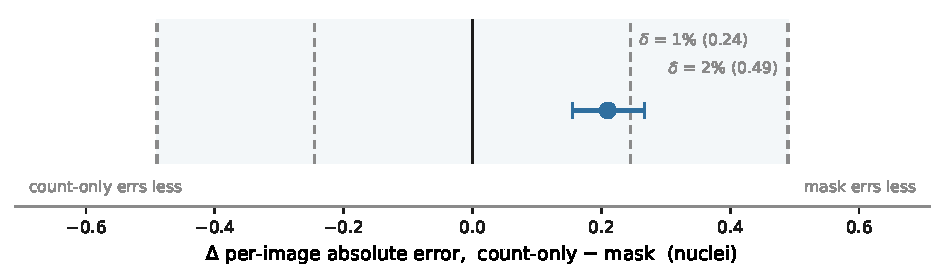
\includegraphics[width=0.85\textwidth]{fig_equivalence.pdf}
\caption{Hiệu số sai số tuyệt đối theo từng ảnh giữa hai chế độ giám sát trên PanNuke fold~3 ($n=2722$), kèm
khoảng tin cậy bootstrap $90\%$, đặt cạnh các biên tương đương $\delta$ biểu diễn theo tỉ lệ số nhân trung bình
mỗi ảnh. Khoảng tin cậy không chứa $0$ nên hiệu số là thật; đồng thời nó nằm gọn trong biên $2\%$ nên hiệu số bị
chặn trên ở mức đó. Biên nhỏ nhất còn cho kết luận tương đương là $\delta^\star = 0{,}27$ nhân.}
\label{fig:equivalence}
\end{figure}

Cần lưu ý phạm vi của phép so sánh này: nhánh mặt nạ dùng \emph{cùng} kiến trúc với chỉ-đếm nhằm cô lập ảnh hưởng
của \emph{kiểu giám sát}, nên nó không đo năng lực của một kiến trúc phân đoạn chuyên dụng.
Mục~\ref{sec:paradigm} xử lý câu hỏi đó riêng.

\subsection{Mô hình chỉ-đếm dựa vào bằng chứng gì?}\label{sec:fidelity}

Kết quả ở Mục~\ref{sec:parity} cho thấy việc bỏ giám sát không gian chỉ làm thay đổi độ chính xác đếm trong một
biên hẹp trên bộ dữ liệu lớn nhất, nhưng chúng không nói mô hình dùng bằng chứng gì để đếm. Một mô hình chỉ thấy
một con số cho mỗi ảnh về nguyên tắc có thể khai thác các tương quan toàn cục (loại mô, mật độ tế bào, đặc trưng
nhuộm) thay vì chính các nhân. Hai phân tích dưới đây kiểm định khả năng đó trên PanNuke fold~3 ($n=2722$ mảnh, số
đếm trung bình $24{,}5$).

\paragraph{Độ chính xác được giữ trên cả 19 loại mô} Các phân tích dưới đây dùng ba mô hình chỉ-đếm được huấn
luyện độc lập theo giao thức ở Mục~\ref{sec:setup}, từ một lần huấn luyện tách khỏi các mô hình của
Bảng~\ref{tab:parity}; mô hình dùng cho Bảng~\ref{tab:perorgan} và Hình~\ref{fig:agreement} đạt $R^2 = 0{,}934$ và
MAE $3{,}40$ trên toàn tập kiểm tra. Các dự đoán nằm sát đường đếm chính xác trên toàn dải số đếm
(Hình~\ref{fig:agreement}a). Chia theo loại mô (Bảng~\ref{tab:perorgan}), $R^2$ dương ở \emph{tất cả} $19/19$
loại, trải từ $0{,}704$ (buồng trứng, $n=52$) tới $0{,}976$ (cổ tử cung, $n=86$). Hai giá trị thấp nhất rơi vào
các loại mô có ít mảnh kiểm tra, nơi ước lượng $R^2$ kém ổn định, nhưng quan hệ này không đơn điệu: loại mô có ít
mảnh nhất (tuỵ, $n=28$) vẫn đạt $0{,}901$, trong khi giá trị thấp thứ ba lại thuộc về một loại có nhiều mẫu
(tuyến thượng thận, $n=155$, $R^2 = 0{,}818$). Phân tích Bland--Altman cho độ chệch $+0{,}70$ nhân, khoảng $3\%$
số đếm trung bình, với giới hạn tương hợp $\pm10{,}2$ nhân (Hình~\ref{fig:agreement}b), nghĩa là sai số không mang
độ chệch có hướng một cách hệ thống. Vậy độ chính xác tổng thể không đến từ việc khớp tốt một vài loại mô chiếm đa
số.

\begin{figure}[!htbp]
\centering
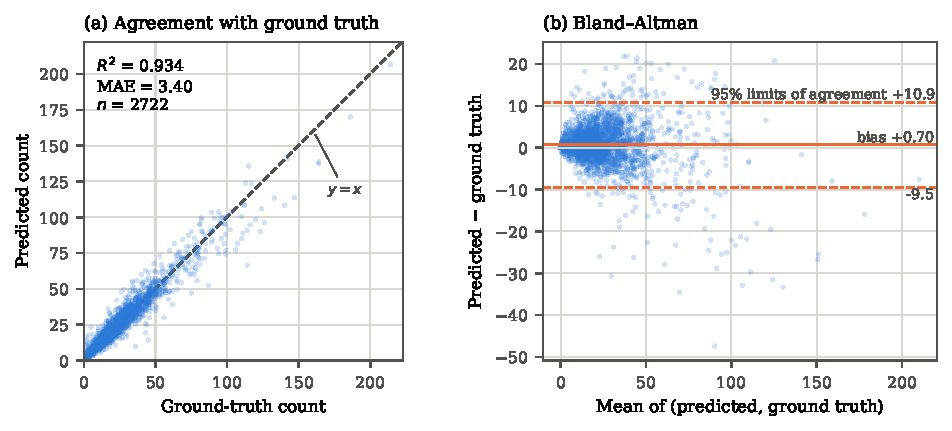
\includegraphics[width=\textwidth]{fig_agreement.pdf}
\caption{Mức tương hợp giữa số nhân dự đoán và số nhân thật của mô hình chỉ-đếm trên PanNuke fold~3 ($n=2722$
mảnh). \textbf{(a)} Mỗi điểm là một mảnh; đường đứt nét là đếm chính xác. \textbf{(b)} Đồ thị Bland--Altman với độ
chệch trung bình và giới hạn tương hợp $95\%$. Độ tản xuống dưới ở các mảnh có số đếm cao cho thấy xu hướng
\emph{đếm thiếu} nhẹ ở chế độ mật độ rất cao.}
\label{fig:agreement}
\end{figure}

\begin{table}[!htbp]
\centering
\caption{Độ chính xác đếm theo từng loại mô trên PanNuke fold~3, cho \emph{một} trong ba mô hình chỉ-đếm ở
Mục~\ref{sec:fidelity} (Hình~\ref{fig:agreement} vẽ cùng mô hình này), có kèm hàng tổng.
Bảng~\ref{tab:parity} báo các con số đã tổng hợp theo seed từ một lần huấn luyện khác, nên hai hàng tổng không
trùng nhau.}\label{tab:perorgan}
\small
\setlength{\tabcolsep}{4pt}
\begin{tabular}{@{}lccc@{\hspace{1.5em}}lccc@{}}
\toprule
Loại mô & $n$ & $R^2$ & MAE & Loại mô & $n$ & $R^2$ & MAE \\
\midrule
Tuyến thượng thận & $155$ & $0{,}818$ & $2{,}43$ & Phổi          & $51$  & $0{,}957$ & $3{,}61$ \\
Ống mật           & $158$ & $0{,}942$ & $2{,}71$ & Buồng trứng   & $52$  & $0{,}704$ & $4{,}31$ \\
Bàng quang        & $64$  & $0{,}924$ & $2{,}34$ & Tuỵ           & $28$  & $0{,}901$ & $3{,}29$ \\
Vú                & $775$ & $0{,}932$ & $2{,}65$ & Tiền liệt tuyến & $68$ & $0{,}756$ & $4{,}43$ \\
Cổ tử cung        & $86$  & $0{,}976$ & $2{,}20$ & Da            & $41$  & $0{,}943$ & $5{,}72$ \\
Đại tràng         & $494$ & $0{,}923$ & $3{,}93$ & Dạ dày        & $48$  & $0{,}963$ & $3{,}95$ \\
Thực quản         & $141$ & $0{,}897$ & $3{,}19$ & Tinh hoàn     & $57$  & $0{,}949$ & $3{,}05$ \\
Đầu \& cổ         & $145$ & $0{,}954$ & $3{,}17$ & Tuyến giáp    & $62$  & $0{,}873$ & $3{,}30$ \\
Thận              & $41$  & $0{,}958$ & $4{,}51$ & Tử cung       & $163$ & $0{,}907$ & $6{,}70$ \\
Gan               & $93$  & $0{,}884$ & $3{,}39$ & \textbf{Tổng} & $2722$ & $0{,}934$ & $3{,}40$ \\
\bottomrule
\end{tabular}
\end{table}

\paragraph{Xoá nhân có đối chứng giả} Để kiểm định quan hệ nhân quả, một tỉ lệ $k$ số nhân đã được chú thích bị
xoá khỏi ảnh và số đếm dự đoán được đo lại. Mỗi nhân được thay bằng một mảnh mô \emph{khớp hình dạng} lấy từ một
vị trí không có nhân trong cùng ảnh đó, và mặt nạ nhân được giãn nở $2$ điểm ảnh trước khi xoá để phủ cả viền nhân
mà chú thích thường bỏ sót. Thao tác này giữ nguyên thống kê kết cấu của mô trong khi loại bỏ nội dung nhân. Đối
chứng giả áp \emph{đúng} thao tác đó với cùng số vùng, cùng hình dạng và cùng diện tích, nhưng ở các vị trí không
có nhân. Nó tách ảnh hưởng của bản thân việc thay thế mô khỏi ảnh hưởng của việc mất nhân. Chỉ những phép đo có
diện tích bị xoá khớp nhau ít nhất $80\%$ giữa hai điều kiện mới được đưa vào các kiểm định thống kê.

\begin{figure}[!htbp]
\centering
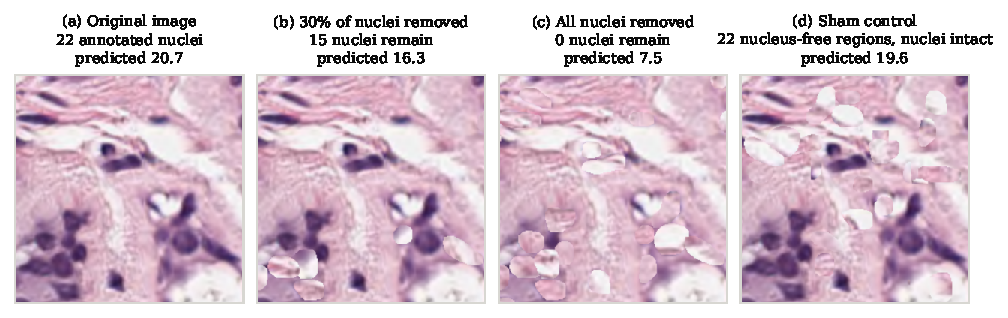
\includegraphics[width=\textwidth]{fig_qualitative.pdf}
\caption{Xoá nhân trên một mảnh PanNuke tiêu biểu (hệ số đáp ứng riêng của nó là $0{,}65$ so với trung bình toàn
bộ dữ liệu $0{,}64$). \textbf{(a)} Ảnh gốc, $22$ nhân đã chú thích. \textbf{(b, c)} Sau khi xoá $30\%$ rồi toàn bộ
số nhân đã chú thích, số đếm dự đoán giảm tương ứng ($20{,}7 \rightarrow 16{,}3 \rightarrow 7{,}5$).
\textbf{(d)} Đối chứng giả trên $22$ vùng \emph{không có nhân}: ảnh bị can thiệp thấy rõ, nhưng số đếm gần như
không đổi ($19{,}6$). Vài nhân sẫm màu còn lại ở (c) là những nhân không có trong chú thích.}
\label{fig:qualitative}
\end{figure}

Số đếm dự đoán giảm \emph{đơn điệu} theo tỉ lệ nhân bị xoá, trong khi đối chứng giả để số đếm gần như không đổi
($1{,}00$--$1{,}02$) ở mọi mức (Bảng~\ref{tab:doseresp}; Hình~\ref{fig:qualitative} minh hoạ thao tác trên một
mảnh). Trên các phép đo khớp diện tích ($n=3415$), phần giảm quy cho nhân là $0{,}234$ đơn vị đã chuẩn hoá và
chiếm trọn phần giảm quan sát được (Wilcoxon bắt cặp giữa hai điều kiện, $p<10^{-300}$). Kết luận không đổi khi
chỉ xét các liều nhỏ ($\le 30\%$), nơi ảnh còn gần phân phối huấn luyện nhất. Vậy đáp ứng là \emph{đặc hiệu} với
nhân chứ không phải với thao tác chỉnh sửa ảnh nói chung.

\begin{table}[!htbp]
\centering
\caption{Đáp ứng của số đếm dự đoán khi xoá nhân, đối chiếu với đối chứng giả xoá một diện tích mô không có nhân
tương đương. Các giá trị được chuẩn hoá theo số đếm trên ảnh nguyên vẹn, lấy trung bình trên $286$ ảnh ($4862$
phép đo) rồi trên $3$ mô hình huấn luyện độc lập; độ lệch chuẩn báo cáo là độ lệch giữa ba mô hình đó. ``Hệ số đáp
ứng'' là phần giảm quan sát được chia cho phần giảm của một bộ đếm kiểm đếm trung thực; giá trị $1{,}0$ ứng với
kiểm đếm trung thực.}\label{tab:doseresp}
\footnotesize
\setlength{\tabcolsep}{5pt}
\begin{tabular}{@{}cccccc@{}}
\toprule
Tỉ lệ bị xoá & Xoá nhân & Đối chứng giả & Phần giảm quy cho nhân & Khớp diện tích & Hệ số đáp ứng \\
\midrule
$10\%$  & $0{,}938\pm0{,}002$ & $1{,}003$ & $0{,}065$ & $0{,}94$ & $0{,}62$ \\
$20\%$  & $0{,}872\pm0{,}004$ & $1{,}004$ & $0{,}131$ & $0{,}91$ & $0{,}64$ \\
$30\%$  & $0{,}805\pm0{,}012$ & $1{,}007$ & $0{,}202$ & $0{,}89$ & $0{,}65$ \\
$50\%$  & $0{,}678\pm0{,}014$ & $1{,}011$ & $0{,}333$ & $0{,}84$ & $0{,}64$ \\
$75\%^{\ast}$  & $0{,}519\pm0{,}020$ & $1{,}012$ & $0{,}494$ & $0{,}78$ & $0{,}64$ \\
$100\%^{\ast}$ & $0{,}374\pm0{,}051$ & $1{,}018$ & $0{,}644$ & $0{,}73$ & $0{,}63$ \\
\bottomrule
\end{tabular}

\vspace{4pt}
\begin{minipage}{\textwidth}\footnotesize
$^{\ast}$ Ở các liều cao, mô bệnh học dày đặc nhân không còn đủ chỗ trống để đặt các vùng đối chứng giả không
chồng lấn, nên diện tích bị xoá của hai điều kiện chỉ khớp tới $0{,}74$--$0{,}78$; các mức này được báo cáo mang
tính mô tả và bị loại khỏi các kiểm định thống kê, vốn chỉ dùng các phép đo khớp diện tích ít nhất $80\%$. Ngoài
ra, xoá toàn bộ nhân là can thiệp lên khoảng $25\%$ diện tích ảnh và do đó gây dịch chuyển phân phối đáng kể; vì
vậy các liều nhỏ được coi là bằng chứng chính.
\end{minipage}
\end{table}

Tuy nhiên đáp ứng lại \emph{dưới tuyến tính} một cách nhất quán: tỉ số giữa phần giảm quan sát được và phần giảm
của một bộ đếm kiểm đếm trung thực nằm trong khoảng $0{,}62$ tới $0{,}65$ ở \emph{mọi} liều từ $10\%$ tới $100\%$
(cột cuối Bảng~\ref{tab:doseresp}), và trung bình là $0{,}64 \pm 0{,}04$ trên ba mô hình huấn luyện độc lập. Xoá
một nhân chỉ làm số đếm giảm khoảng $0{,}6$ thay vì $1{,}0$. Phần hụt này là một hệ số cố định, không phải hiệu
ứng bão hoà ở liều cao.

Cách diễn giải nhất quán nhất là mô hình \emph{tích hợp bằng chứng liên quan tới nhân trên toàn ảnh} chứ không
phát hiện rồi kiểm đếm từng thực thể. Một phép đo độc lập ủng hộ cách đọc này: bản đồ mật độ của mô hình chỉ-đếm
\emph{gần như không} định vị nhân. Khối lượng mật độ rơi vào vùng nhân thật chỉ gấp $1{,}25\pm0{,}36$ lần so với
một bản đồ đều ($1{,}0$ ứng với hoàn toàn không định vị), nên độ lệch so với mốc không-định-vị còn nhỏ hơn biến
thiên giữa các seed; và tương quan không gian với bản đồ mật độ chuẩn chỉ là $0{,}03$ (ba seed), gần mức ngẫu
nhiên. Mốc đối chiếu ở đây là một bản đồ không mang thông tin vị trí, chứ không phải khả năng định vị của một mô
hình được giám sát dày đặc, thứ mà bài báo không đo. Hai quan sát này nhất quán với một lời giải thích duy nhất,
và nó lý giải vì sao giám sát mức ảnh đủ cho việc \emph{đếm} mà không sinh ra khả năng định vị: đại lượng được
giám sát là một tổng, nên nghiệm mà mô hình tìm ra chỉ cần đúng ở mức tổng.

Ba kiểm tra bổ sung cho thấy phần hụt này không phải là hiện vật của cách thiết kế phép xoá; cả ba đều chạy trên
\emph{một} mô hình chỉ-đếm, nên nên được đọc như những khác biệt giữa các cấu hình. Thứ nhất, giãn nở mặt nạ $0$,
$2$ và $4$ điểm ảnh trước khi xoá, tương ứng diện tích bị can thiệp $18\%$, $25\%$ và $31\%$ ảnh, cho các hệ số
$0{,}59$, $0{,}60$ và $0{,}61$; toàn bộ dải này còn nhỏ hơn độ lệch giữa các mô hình, nên việc phủ chưa hết viền
nhân không giải thích được phần hụt. Thứ hai, những nhân bị chú thích bỏ sót không bị xoá nên vẫn đóng góp vào số
đếm: số đếm dư sau khi xoá hết nhân đã chú thích tăng đơn điệu từ $0{,}36$ ở nhóm mảnh không có dấu hiệu bỏ sót
lên $0{,}70$ ở nhóm bỏ sót nhiều nhất (tương quan $+0{,}31$, $n = 286$), nhưng phần dự đoán vượt quá số đếm đã chú
thích chỉ trung bình khoảng $3{,}5\%$ so với số đếm dư $37{,}4\%$, nên phần lớn khoảng cách tới $1{,}0$ không thể
quy cho chất lượng chú thích. Ngược lại, phép đo \emph{có} nhạy với cách lấp vùng bị xoá: thay ghép mảnh bằng nội
suy Telea ở cùng mức giãn nở làm hệ số tụt từ $0{,}59$ xuống $0{,}34$, vì nội suy lan màu vào trong từ biên vùng
cần lấp, mà biên đó chính là viền nhân, nên nó để lại dấu vết nhân trong ảnh. Vậy hệ số đo được bị chặn trên bởi
mức triệt để của phép xoá, và $0{,}64$ là một cận dưới của độ nhạy thật.

\subsection{So sánh với các phương pháp dùng nhãn định vị}\label{sec:paradigm}

Bộ đếm chỉ-đếm nhẹ đạt $R^2$ và MAE tốt hơn cả ba đại diện được khảo sát của phân đoạn, ước lượng mật độ và phát
hiện, dù chỉ dùng nhãn đếm (Bảng~\ref{tab:paradigm}). Mỗi mô thức chỉ được đại diện bởi \emph{một} phương pháp,
nên kết quả này nói về các phương pháp cụ thể đã khảo sát chứ không về giới hạn của cả một hướng tiếp cận. Cả bốn
phương pháp đều được huấn luyện lại và đánh giá trên cùng tập kiểm tra ở mức tác vụ đếm. Số đếm của mỗi phương
pháp so sánh được lấy qua chính hậu xử lý chính thức của nó: số thực thể sau khi tách với StarDist, số cực đại địa
phương trên bản đồ mật độ trọng tâm với DualU-Net, và số điểm còn lại sau triệt phi cực đại với DeNuC. Khác với
phép so sánh có đối chứng ở Mục~\ref{sec:parity}, ở đây kiến trúc, số tham số và siêu tham số đều khác nhau giữa
các phương pháp, nên kết quả cho biết các mô thức này hành xử ra sao ở cấu hình thông dụng của chúng trên tác vụ
đếm, chứ không cô lập được một nguyên nhân duy nhất.

Phương pháp phát hiện suy giảm đơn điệu theo mật độ nhân: độ chệch số đếm tăng từ $-0{,}8$ trên các mảnh thưa lên
$-30{,}4$ trên các mảnh có từ $45$ nhân trở lên. Diễn tiến này khớp với cơ chế mà triệt phi cực đại loại bỏ các
trường hợp dương thật khi các nhân chồng lấn, và giải thích vì sao hồi quy số đếm chiếm ưu thế ở chế độ mật độ
cao.

\begin{table}[!htbp]
\centering
\caption{So sánh bốn mô thức trên PanNuke (cùng tập kiểm tra, tác vụ đếm). DensitySigmaUNet báo trung bình và độ
lệch chuẩn trên $5$ seed, đúng các con số ở Bảng~\ref{tab:parity}, và StarDist đã được huấn luyện lại trên cùng
$5$ seed đó; DualU-Net và DeNuC mỗi phương pháp chỉ có một lần huấn luyện, nên khác biệt liên quan đến chúng nên
được đọc đối chiếu với mức biến thiên giữa các seed nêu ở những hàng có con số đó. Giá trị tốt nhất mỗi cột được in đậm.}\label{tab:paradigm}
\small
\begin{tabular}{@{}lccccc@{}}
\toprule
Phương pháp & Tham số & Nhãn & Mô thức & $R^2\uparrow$ & MAE$\downarrow$ \\
\midrule
DensitySigmaUNet & $3{,}62$M & số đếm & hồi quy & $\mathbf{0{,}918\pm0{,}011}$ & $\mathbf{3{,}60\pm0{,}10}$ \\
StarDist~\cite{stardist} & $1{,}43$M & mặt nạ & phân đoạn & $0{,}847\pm0{,}011$ & $4{,}38\pm0{,}05$ \\
DualU-Net~\cite{dualunet} & $41{,}0$M & mặt nạ & mật độ trọng tâm & $0{,}804$ & $5{,}33$ \\
DeNuC~\cite{denuc} & $4{,}37$M & điểm & phát hiện & $0{,}455$ & $9{,}64$ \\
\bottomrule
\end{tabular}
\end{table}

\subsection{Hệ thống đối chiếu với ba ngân sách của nó}\label{sec:deploy}
\subsubsection{Ngân sách chú thích}\label{sec:label}
Một phần tư ngân sách chú thích đã đủ cho khoảng $93\%$ hiệu năng đạt được với toàn bộ nhãn. Trên PanNuke, $R^2$
theo tỉ lệ ảnh được gán nhãn đếm là $0{,}453 \pm 0{,}208$ ở $5\%$, $0{,}742$ ở $10\%$, $0{,}849 \pm 0{,}029$ ở
$25\%$, $0{,}859$ ở $50\%$ và $0{,}915 \pm 0{,}010$ với toàn bộ nhãn (ba seed, cùng giao thức đánh giá; giá trị ở
ngân sách đầy đủ lệch $0{,}003$ so với Bảng~\ref{tab:parity}, nằm trong biến thiên giữa các seed). Đường cong bão
hoà sớm: phần lớn mức tăng được hiện thực trong một phần tư ngân sách đầu tiên, còn đi từ $25\%$ lên $100\%$ chỉ
thêm $0{,}066$. Điểm $5\%$ đánh dấu giới hạn dưới của chế độ này, nơi phương sai giữa các seed lấn át giá trị
trung bình. Với một đợt triển khai, điều này nghĩa là hợp đồng chú thích có thể được định lượng thấp hơn hẳn mức
phủ toàn bộ, và giá trị biên của mỗi ảnh gán nhãn thêm là đo được trước chứ không phải phỏng đoán.

\subsubsection{Chi phí chú thích theo từng kiểu nhãn và ngân sách tính toán}\label{sec:cost}
Khác biệt lớn hơn nằm ở phía chú thích. Qu và cộng sự~\cite{qu2020} cho một bác sĩ giải phẫu bệnh chú thích tám
ảnh theo ba cách khác nhau và đo thời gian: với các ảnh chứa trung bình khoảng $600$ nhân, khoanh viền đầy đủ mất
khoảng $115$ phút, hộp bao mất khoảng $67$ phút, còn đặt một điểm lên mỗi nhân chỉ mất khoảng $14$ phút. Chi phí
của nhãn đếm mức ảnh chưa được đo trực tiếp trong tài liệu, nhưng nó bị chặn trên bởi chi phí đánh dấu điểm: đếm
đòi hỏi quét qua các nhân đúng như khi đánh dấu điểm, mà không phải đặt từng điểm cho chính xác và không phải
khoanh viền gì cả. Theo các con số đó, nhãn đếm rẻ hơn ít nhất $8$ lần so với mặt nạ đầy đủ, và một số đếm gần
đúng còn rẻ hơn nữa. Tỉ lệ này nên được hiểu là một bậc độ lớn chứ không phải một hằng số chuyển giao được: nó dựa
trên tám ảnh của một người chú thích duy nhất, và những ảnh đó dày đặc hơn nhiều so với các mảnh $256\times256$
dùng ở đây (trung bình $24{,}5$ nhân). Thứ được bảo toàn giữa hai chế độ là chi phí \emph{trên mỗi nhân}: cũng
theo các con số đó, khoanh viền tốn khoảng $11{,}5$ giây mỗi nhân và đánh dấu điểm khoảng $1{,}4$ giây, còn đếm
thì không thể đắt hơn đánh dấu. Đặt cạnh phần mất mát độ chính xác đo được ở Mục~\ref{sec:parity}, bị chặn trên ở
khoảng $1\%$ số nhân mỗi ảnh, sự bất đối xứng này là luận điểm hiệu quả trung tâm của bài báo.

Về phía tính toán, bộ đếm có $3{,}62$M tham số và $0{,}98$ GMACs ở đầu vào $256\times256$, độ trễ $6{,}0$\,ms
trên GPU và $46$\,ms trên CPU, và bộ nhớ đỉnh $37{,}9$\,MB. Các con số này cho phép suy luận thời gian thực trên
cả GPU phổ thông lẫn CPU, nên hệ đã triển khai không đòi hỏi phần cứng tăng tốc chuyên dụng. So sánh ở
Bảng~\ref{tab:paradigm} cho thấy điều này không đạt được bằng cách đánh đổi độ chính xác lấy kích thước: bộ đếm
nhỏ hơn $11{,}3$ lần so với phương pháp lớn nhất được so sánh mà vẫn chính xác hơn trên tác vụ đếm.

\subsubsection{Đặc tả độ tin cậy}\label{sec:uq}
Các khoảng dự báo được hiệu chuẩn không chỉ theo biên mà còn có điều kiện theo cơ quan (Bảng~\ref{tab:uq}). Cả ba
sơ đồ đều đạt độ phủ biên mục tiêu $0{,}90$, nhưng chỉ mondrian nâng được độ phủ của cơ quan bị phủ kém nhất lên
đúng mức mục tiêu đó ($0{,}906$), trong khi một ngưỡng dùng chung để bốn trong số $19$ loại mô nằm dưới ngưỡng
dung sai. Cái giá là khoảng rộng hơn khoảng $15\%$. Chính sự phân biệt này biến một con số trung bình thành một
đặc tả dùng được: một hệ có dung sai đúng trên tổng thể nhưng hỏng ở bốn trên mười chín loại mô thì không thể được
chứng nhận cho các loại mô đó, và mức phạt $15\%$ bề rộng là cái giá để loại bỏ kiểu hỏng ấy.

Các độ phủ quan sát được không phải tham số tự do: cả ba đều suy ra từ Phương trình~\eqref{eq:cov} và kích thước
các nhóm hiệu chuẩn, không khớp gì cả. Nửa hiệu chuẩn của fold~3 có $n = 1361$ ảnh, cho độ phủ global dự báo
$k/(n+1) = 0{,}901$ so với $0{,}904$ quan sát được. Dưới sơ đồ mondrian, cũng những ảnh đó được chia theo cơ quan
thành các nhóm từ $n_g = 14$ (tuỵ) tới $387$ (vú); nhóm duy nhất nằm dưới ngưỡng $15$, vốn là một biên an toàn so
với chặn khả thi ở Phương trình~\eqref{eq:feas}, quay về dùng $q$ chung, và trung bình có trọng số theo kích thước
của $k_g/(n_g+1)$ trên mười tám nhóm còn lại là $0{,}919$, so với $0{,}923$ quan sát được. Với sơ đồ cluster, ba
nhóm gộp đủ lớn để dự báo là $0{,}903$ bất kể cơ quan nào được gộp với nhau, biến thiên dưới $0{,}001$ trên mọi
cách gán mười chín cơ quan vào ba nhóm, so với $0{,}906$ quan sát được. Vậy mỗi dự báo đều nằm trong $0{,}004$ so
với phép đo, và phần dư đều dương ở cả ba trường hợp, đúng như dự kiến: khoảng bị cắt cận dưới tại không và các
điểm số dễ trùng nhau vì số đếm là số nguyên, cả hai hiệu ứng đều chỉ có thể nâng độ phủ lên trên chặn ở
Phương trình~\eqref{eq:cov}.

Đó là ý nghĩa theo đó việc mondrian phủ dư, $0{,}923$ so với mục tiêu $0{,}90$, không phải một khiếm khuyết của
hiệu chuẩn mà là cái giá của bảo đảm có điều kiện. Chia $1361$ ảnh hiệu chuẩn thành mười chín nhóm cơ quan làm
phần dư $1/(n_g+1)$ ở Phương trình~\eqref{eq:cov} lớn lên khoảng mười chín lần, và chính phần dư đó, chứ không
phải một $\sigma$ sai hiệu chuẩn, sinh ra cả phần phủ dư lẫn $15\%$ bề rộng thêm. Thứ mà một đợt triển khai mua
được bằng bề rộng ấy nằm ở cột cuối của Bảng~\ref{tab:uq}.

Việc neo $\sigma$ vào mức nền phương sai Poisson có ý nghĩa khi dải số đếm rộng. Trên NuInsSeg, nơi số đếm mỗi ảnh
trải từ vài nhân tới hơn $500$, dạng neo Poisson cho bề rộng khoảng $37{,}7$ so với $67{,}9$ của $\sigma$ không
neo ($-44\%$), điểm Winkler $45{,}4$ so với $78{,}1$ ($-42\%$), và độ phủ cơ quan kém nhất $0{,}864$ so với
$0{,}655$, ở cùng độ phủ biên khoảng $0{,}93$. Trên PanNuke, nơi số đếm tập trung trong một dải hẹp, hai dạng
không khác nhau đáng kể. Vậy neo Poisson là một lựa chọn thiết kế cho dữ liệu dải rộng chứ không phải một cải
thiện đồng đều. Đầu $\sigma$ không làm giảm độ chính xác đếm, vì $\mu$ được tách khỏi nhánh bất định.

\begin{table}[!htbp]
\centering
\caption{Chất lượng khoảng dự báo sau hiệu chuẩn conformal trên PanNuke fold~3 ($n=2722$), lấy trung bình trên
$20$ lần chia hiệu chuẩn ngẫu nhiên. Độ phủ mục tiêu là $0{,}90$; bề rộng và điểm Winkler tính theo đơn vị nhân,
thấp hơn là tốt hơn. Một loại mô bị tính là thiếu phủ khi độ phủ của nó thấp hơn mục tiêu quá $0{,}05$, tức dưới
$0{,}85$; dung sai này giải thích vì sao sơ đồ cluster có độ phủ cơ quan kém nhất là $0{,}859$ mà vẫn không loại
mô nào bị tính là thiếu phủ. Giá trị tốt nhất mỗi cột được in đậm, trừ độ phủ biên vốn là một kiểm tra tính hợp lệ
đối chiếu với mục tiêu $0{,}90$ chứ không phải đại lượng cần tối đa hoá.}\label{tab:uq}
\footnotesize
\setlength{\tabcolsep}{5pt}
\begin{tabular}{@{}lccccc@{}}
\toprule
Sơ đồ & Độ phủ biên & Bề rộng & Winkler & Độ phủ cơ quan kém nhất & Số cơ quan thiếu phủ \\
\midrule
global & $0{,}904$ & $\mathbf{14{,}5}$ & $20{,}3$ & $0{,}765$ & $4/19$ \\
mondrian & $0{,}923$ & $16{,}6$ & $20{,}5$ & $\mathbf{0{,}906}$ & $\mathbf{0/19}$ \\
cluster & $0{,}906$ & $14{,}8$ & $\mathbf{20{,}0}$ & $0{,}859$ & $\mathbf{0/19}$ \\
\bottomrule
\end{tabular}
\end{table}

%%============================================================%%
\section{Thảo luận}\label{sec:discuss}

\paragraph{Vì sao giám sát mức ảnh có thể là đủ cho bài toán đếm nhân} Các thí nghiệm can thiệp đưa ra một lời
giải thích hợp lý cho việc thông tin vị trí chi tiết không phải là thành phần quyết định của độ chính xác đếm. Số
đếm dự đoán giảm đúng khi các nhân bị xoá khỏi ảnh nhưng gần như không đổi dưới các can thiệp giả khớp diện tích;
đồng thời đáp ứng vẫn dưới tuyến tính và bản đồ mật độ học được hầu như không mang thông tin vị trí. Hai quan sát
này nhất quán với giả thuyết rằng mô hình học cách tích hợp bằng chứng liên quan tới nhân trên toàn ảnh chứ không
phải phát hiện rồi kiểm đếm từng thực thể. Nếu vậy, một nhãn đếm mức ảnh có thể đã cung cấp phần lớn thông tin cần
cho tác vụ đếm.

\paragraph{Hệ quả cho thiết kế} Đọc đối chiếu với ba ngân sách ở Mục~\ref{sec:intro}, các phép đo cho ra một hệ
rẻ trên cả ba trục cùng lúc. Hợp đồng chú thích có thể viết cho nhãn đếm mức ảnh, rẻ hơn ít nhất tám lần mỗi ảnh
so với khoanh viền đầy đủ, và định lượng ở khoảng một phần tư mức phủ toàn bộ để đạt khoảng $93\%$ độ chính xác
khả dĩ. Chi phí suy luận nằm trong mức mà một CPU phục vụ được theo thời gian thực, nên hệ không áp đặt phần cứng
tăng tốc lên cơ sở triển khai nó. Yêu cầu độ tin cậy được đáp ứng bằng hiệu chuẩn conformal có điều kiện theo cơ
quan, vốn là một thủ tục hậu nghiệm nên không ràng buộc cách bản thân bộ đếm được huấn luyện. Đại lượng duy nhất
phải đánh đổi bị chặn trên ở khoảng $1\%$ số nhân mỗi ảnh trên bộ dữ liệu lớn nhất đã kiểm tra. Chính sự bất đối
xứng này, chứ không phải một con số độ chính xác riêng lẻ nào, mới là thứ khiến thiết kế chỉ-đếm là lựa chọn hợp
lý khi đầu ra cần có là số đếm.

\paragraph{Chuyển giao ngoài miền} Cơ chế tích hợp bằng chứng toàn ảnh cũng gợi ra một hạn chế tiềm tàng. Vì mô
hình học các tín hiệu liên quan tới nhân ở một thang không gian nhất định, độ chính xác có thể suy giảm khi độ
phóng đại hoặc kích thước nhân biểu kiến khác biệt đáng kể giữa miền huấn luyện và miền triển khai. Ngược lại, các
khoảng dự báo conformal không giả định dạng phân phối nào: sau khi hiệu chuẩn lại trên một tập hiệu chuẩn nhỏ từ
miền đích, độ phủ mong muốn vẫn được giữ dưới giả thiết khả hoán ngay cả khi độ chính xác điểm thay đổi. Khi đó
khoảng nới rộng ra đóng vai trò tín hiệu cảnh báo rằng một mẫu nằm ngoài vùng mà mô hình còn đáng tin.

\paragraph{Hạn chế và phạm vi} Nghiên cứu này được thiết kế như một thí nghiệm có đối chứng nhằm cô lập vai trò
của kiểu giám sát. Do đó các kết luận của nó được thiết lập trên một họ kiến trúc duy nhất, một bộ mã hoá nhẹ ghép
với một bộ giải mã kiểu U-Net. Việc các quan sát tương tự có còn đúng trên những kiến trúc khác, chẳng hạn mô hình
transformer hay các hệ phân đoạn nhân chuyên dụng, vẫn cần được kiểm chứng bằng thực nghiệm. Ngoài ra, vì nhánh
mặt nạ dùng chính kiến trúc của bộ đếm, phép so sánh chính đo vai trò của \emph{kiểu giám sát} chứ không thiết lập
được cận trên cho một pipeline phân đoạn được tối ưu riêng; Mục~\ref{sec:paradigm} chỉ lấp được một phần khoảng
trống đó.

Thêm nữa, bài báo chỉ xét tác vụ đếm. Các kết quả không hàm ý rằng giám sát mức ảnh là đủ cho những tác vụ đòi hỏi
thông tin không gian, như phân đoạn thực thể, định vị nhân hay phân tích hình thái. Trái lại, các kết quả can
thiệp cho thấy một mô hình chỉ-đếm không dễ hình thành một biểu diễn có định vị mang ý nghĩa, ngay cả khi nó đếm
chính xác.

\section{Kết luận}\label{sec:conclusion}

Bài báo đã kiểm định trực tiếp vai trò của giám sát không gian trong bài toán đếm nhân, thông qua một thí nghiệm
có đối chứng trong đó kiến trúc, dữ liệu và giao thức đánh giá được giữ cố định và biến duy nhất là kiểu giám sát.
Trên ba bộ dữ liệu bệnh học độc lập, không chế độ nào ưu thế nhất quán; trên PanNuke, lợi thế của giám sát bằng
mặt nạ có ý nghĩa thống kê nhưng bị chặn trên bởi một kiểm định tương đương ở khoảng $1\%$ số nhân trung bình mỗi
ảnh. Trong khi đó, nhãn đếm mức ảnh rẻ hơn ít nhất tám lần so với khoanh viền đầy đủ.

Các thí nghiệm can thiệp cho thấy mô hình chỉ-đếm phản ứng đặc hiệu với nội dung nhân nhưng hình thành dự đoán
bằng cách tích hợp bằng chứng trên toàn ảnh chứ không phải bằng cách định vị từng thực thể, điều này vừa giải
thích độ chính xác đếm đạt được vừa vạch ra giới hạn của nó với các tác vụ cần thông tin không gian. Trên chính
tác vụ đếm, bộ đếm đạt độ chính xác cao hơn cả ba đại diện được khảo sát của các phương pháp dùng nhãn định vị,
chạy thời gian thực trên CPU, và mang theo các khoảng dự báo có điều kiện theo cơ quan giữ được độ phủ mục tiêu
trên mọi loại mô.

Nhìn tổng thể, với bài toán đếm nhân, chú thích không gian dày đặc không phải điều kiện tiên quyết để đạt độ chính
xác cao, và ngân sách chú thích của một hệ định lượng đã triển khai có thể giảm khoảng một bậc độ lớn để đổi lấy
một phần mất mát bị chặn và đo được. Các hướng tiếp theo gồm kiểm chứng kết luận này khái quát tới đâu trên những
họ kiến trúc khác và trên những miền dữ liệu khác biệt đáng kể về độ phân giải, cơ quan và quy trình nhuộm; và
truy tìm những đặc trưng ảnh nào cấu thành phép tích hợp mà bộ đếm học được, bao gồm câu hỏi vì sao hệ số đáp ứng
của nó nhỏ hơn một.

%%============================================================%%
\section*{Phân công đóng góp (CRediT)}
\textbf{Viet Hang Duong:} Hình thành ý tưởng, Phương pháp luận, Thẩm định, Viết -- rà soát và biên tập, Giám sát.
\textbf{Thi Thu Hiep Dinh:} Hình thành ý tưởng, Điều tra nghiên cứu, Phần mềm, Phân tích chính thức, Trực quan
hoá, Viết -- bản thảo gốc.

\section*{Tuyên bố về xung đột lợi ích}
Các tác giả tuyên bố không có lợi ích tài chính hay quan hệ cá nhân nào có thể ảnh hưởng tới công trình được báo
cáo trong bài này.

\section*{Tuyên bố về việc dùng công nghệ AI trong quá trình viết}
Trong quá trình chuẩn bị công trình này, các tác giả có dùng công cụ hỗ trợ bằng AI nhằm cải thiện tính dễ đọc và
ngôn ngữ của bản thảo. Sau khi dùng các công cụ này, các tác giả đã rà soát và biên tập lại nội dung khi cần, và
chịu hoàn toàn trách nhiệm về nội dung của bài báo.

\section*{Tài trợ}
Nghiên cứu này được tài trợ bởi Quỹ Hỗ trợ Nghiên cứu Khoa học của Trường Đại học Công nghệ Thông tin, ĐHQG-HCM.

\section*{Chấp thuận đạo đức}
Không áp dụng. Nghiên cứu chỉ dùng các bộ dữ liệu ảnh bệnh học công khai, đã công bố trước đó và đã khử định danh;
không thu thập dữ liệu mới từ người hay động vật.

\section*{Tính sẵn có của dữ liệu}
Nghiên cứu chỉ dùng dữ liệu công khai: PanNuke~\cite{pannuke}, NuInsSeg~\cite{nuinsseg} và
MoNuSeg~2018~\cite{monuseg}, truy cập được qua các công bố gốc tương ứng. Không có dữ liệu mới nào được tạo ra. Mã
nguồn dùng để huấn luyện, đánh giá và tái lập mọi bảng và hình trong bài sẽ được công khai khi bài được chấp nhận.

\section*{Lời cảm ơn}
Các tác giả cảm ơn Trường Đại học Công nghệ Thông tin, ĐHQG-HCM đã hỗ trợ nghiên cứu này.

\bibliographystyle{elsarticle-num}
\bibliography{references}

\end{document}
